\subsection{Comparación de estrategias binarias: BS y BSII}

Para la comparación de los resultados obtenidos con cada una de las estrategias binarias se registran las métricas de precisión, \textit{recall} y \textit{f1-socre}. Por claridad se indica que en las gráficas siguientes \ref{fig:Precision} a \ref{fig:F1-score} las etiquetas son:
\begin{itemize}
    \item \textbf{BS\_and:} Búsqueda binaria con conjunción.
    \item \textbf{BS\_or:} Búsqueda binaria con disyunción.
    \item \textbf{BS\_II\_and:} Búsqueda binaria con índice invertido con conjunción.
    \item \textbf{BS\_II\_or:} Búsqueda binaria con índice invertido con disyunción.
\end{itemize}

La precisión (véase figura \ref{fig:Precision}) indica qué porcentaje de los documentos recuperados se consideran relevantes de acuerdo con la etiqueta de la consulta. Como se esperaba los resultados de las estrategias con conjunción (AND) son mejores que los de disyunción (OR). Esto debido a que hay una mayor probabilidad de que si el documento contienen todos los términos de la consulta sea relevante, mientras que si contiene solo uno de ellos, la probabilidad es muchísimo menor.\\ 

\begin{figure}
    \centering
    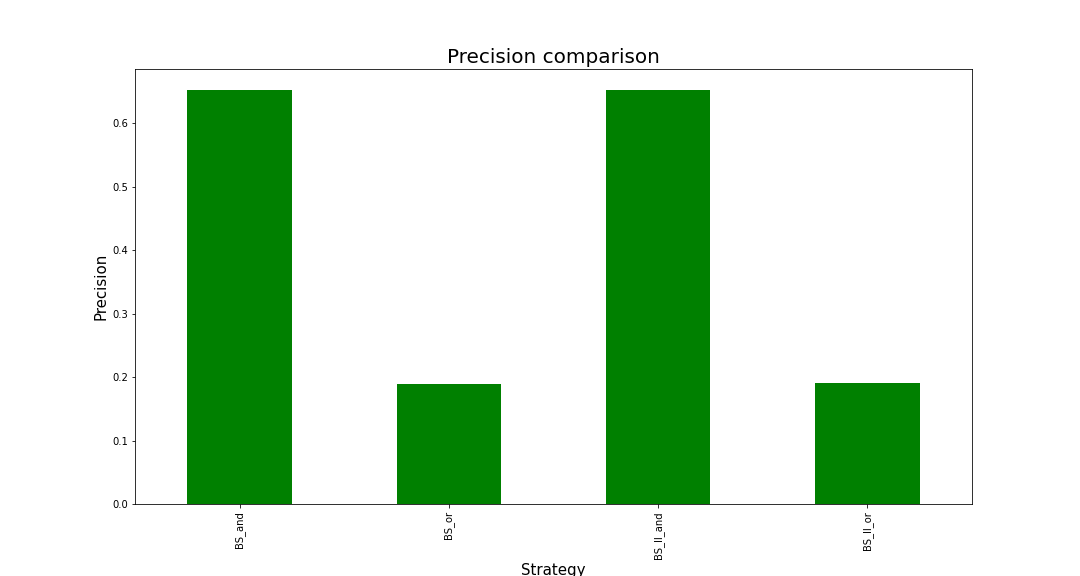
\includegraphics[width=\textwidth]{results/images/BS_precision_comparison.png}
    \caption{Precisión de cada estrategia.}
    \label{fig:Precision}
\end{figure}

El \textit{recall} (véase figura \ref{fig:Recall}), por su parte evalúa qué porcentaje de los documentos relevantes fueron recuperados. Con esto en mente, se espera que el resultado de esta métrica con las estrategias de disyunción sea muy buena, mientras que en las estrategias de conjunción resulta mala. Esto se debe a que existe la posibilidad de que un documento que no contiene todos los términos de la búsqueda sea relevante, por ejemplos sinónimos. Esto ocasiona que la estrategia de conjunción devuelva un valor mucho menor, pues retorna un porcentaje bajo del total de documentos que debería retornar.\\

\begin{figure}
    \centering
    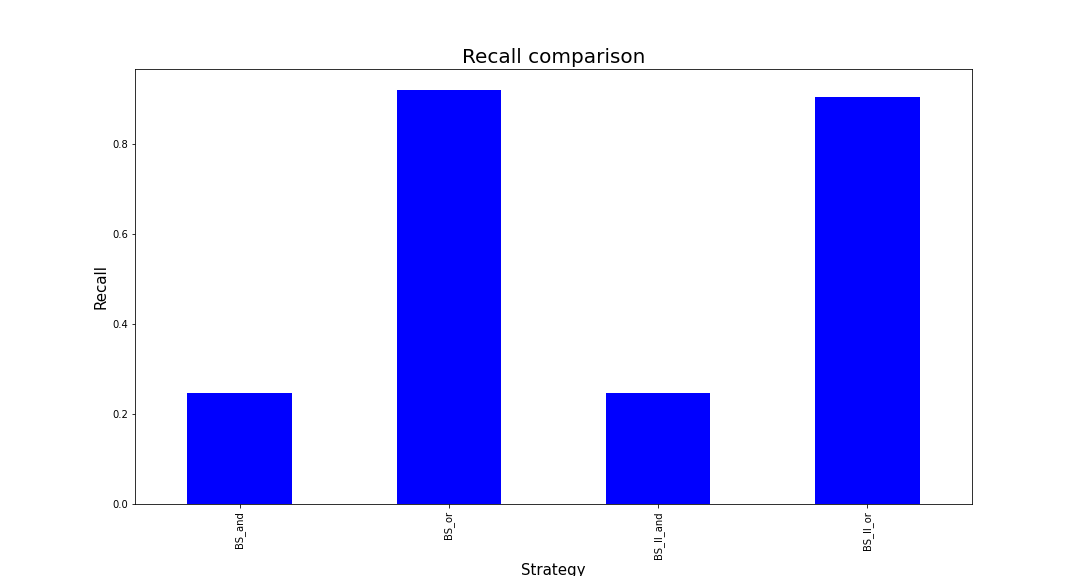
\includegraphics[width=\textwidth]{results/images/BS_recall_comparison.png}
    \caption{\textit{Recall} de cada estrategia.}
    \label{fig:Recall}
\end{figure}

Como se puede observar, las gráficas anteriores evidencian que bajo una de la luz de la métrica de precisión, las estrategias de AND retornan valores muchísimo más altos que los de OR, mientras que para \textit{recall} el resultado de las estrategias disyuntivas son muchísimo mejores. Es por esto que se recurre a una métrica que permita ponderar el resultado de precisión y \textit{recall}. F1-score (véase figura \ref{fig:F1-score}) es una métrica que pondera estos resultados. Se calcula como se muestra en la ecuación \ref{eq:recall}. 

\begin{equation}
    R = \frac{2PR}{P+R}
    \label{eq:recall}
\end{equation}

El resultado es ideal cuando es 1, pues significa que ambas métricas son perfectas. No obstante, es difícil de obtener. El resultado obtenido con las implementaciones actuales indica que el desempeño de las estrategias AND es mejor que el de las OR. Sin embargo, puede resultar conveniente ponderar de manera diferente el peso dado a cada métrica, en caso tal que resulte preferible obtener más documentos relacionados y no únicamente de los que se tenga total certeza de que son relevantes.

\begin{figure}[H]
    \centering
    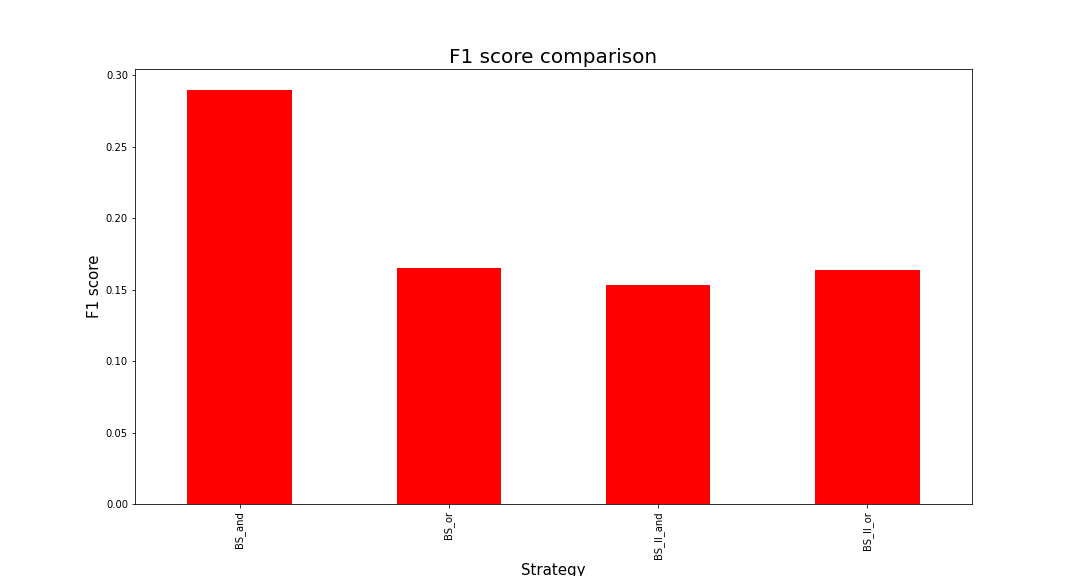
\includegraphics[width=\textwidth]{results/images/BS_f1_comparison.png}
    \caption{F1-score de cada estrategia.}
    \label{fig:F1-score}
\end{figure}


\subsection{Comparación de estrategias clasificadas (\textit{ranked}): RRI, RRDV, GENSIM}

Para evaluar el desempeño de las estrategias de recuperación de la información clasificadas \textit{(ranked)}, se realizó el calculo de las métricas \texttt{P@M}, \texttt{R@M}, \texttt{NDGC@M} y \texttt{MAP} para cada uno de los 35 \textit{queries} en el dataset, donde $M$ representa el número de documentos relevantes en la etiqueta. Para esto se hizo uso de las funciones desarrolladas en la primera parte de este trabajo, las cuales se encuentran en el archivo \texttt{metrics.py}. Como resultado de este proceso se obtuvieron las figuras \ref{fig:rankedP} - \ref{fig:rankedNDCG} y el cuadro \ref{tab:rankedResults} que resume los resultados promedio de todas las estrategias implementadas. \\

En términos generales, se puede observar que los resultados de todas las estrategias \textit{ranked} son bastante buenos. Salvo por dos \textit{queries}, todas las estrategias son capaces de recuperar al menos un documento relevante

\begin{figure}[H]
    \centering
    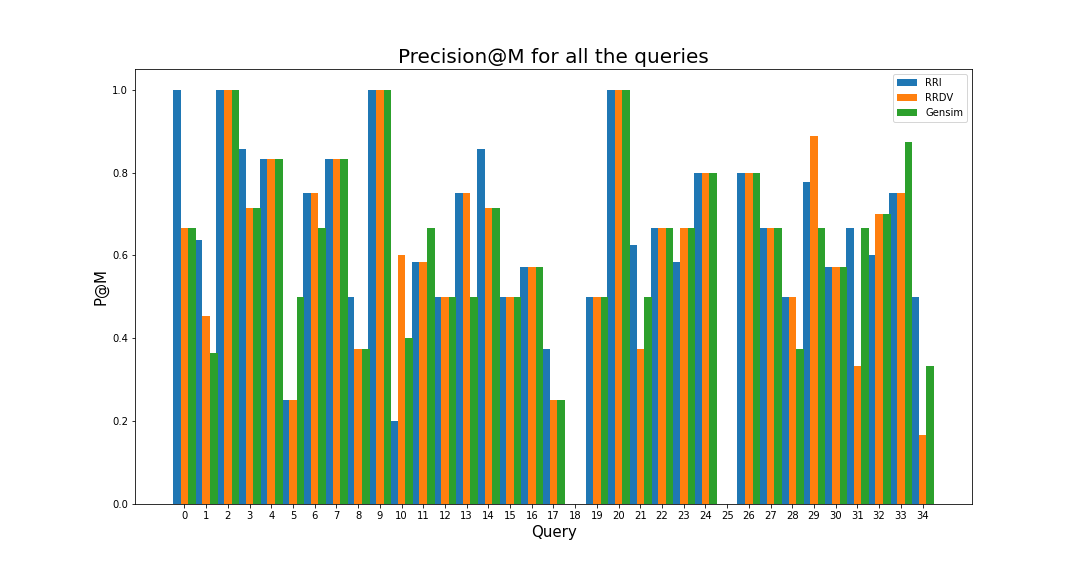
\includegraphics[width=\textwidth]{doc/images/P@M_Ranked.png}
    \caption{Resultados de P@M para todas las queries del data set con las estrategias clasificadas (\textit{ranked})}
    \label{fig:rankedP}
\end{figure}

\begin{figure}[H]
    \centering
    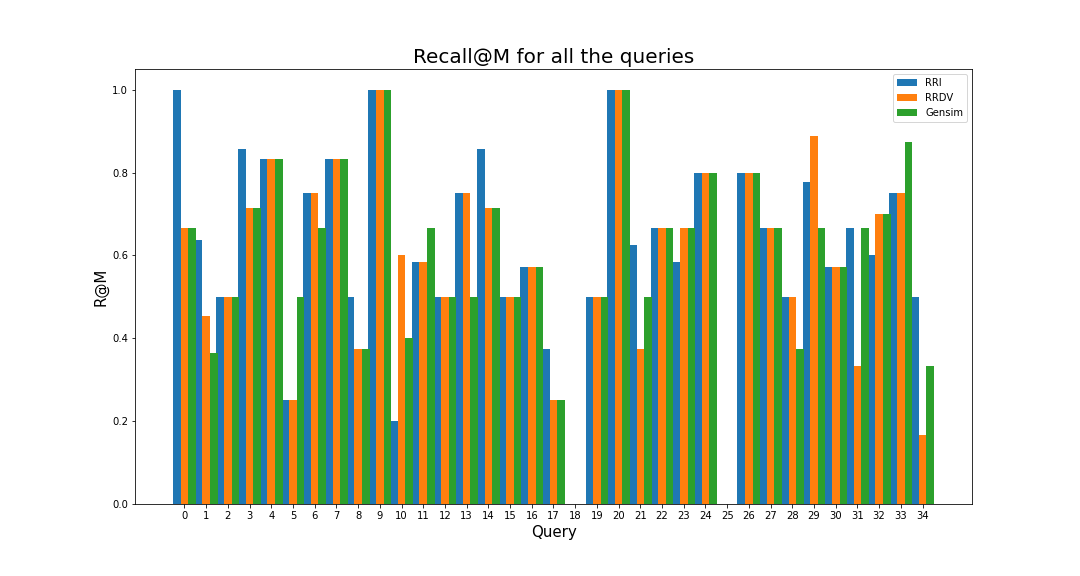
\includegraphics[width=\textwidth]{doc/images/R@M_Ranked.png}
    \caption{Resultados de R@M para todas las queries del data set con las estrategias clasificadas (\textit{ranked})}
    \label{fig:rankedR}
\end{figure}


\begin{figure}[H]
    \centering
    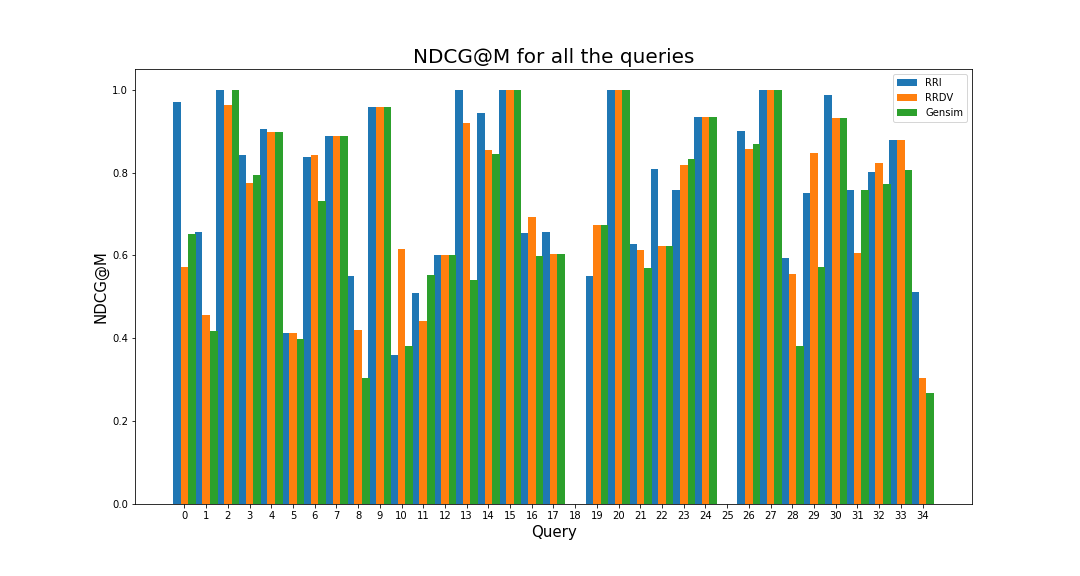
\includegraphics[width=\textwidth]{doc/images/NDCG@M_Ranked.png}
    \caption{Resultados de NDCG@M para todas las queries del data set con las estrategias clasificadas (\textit{ranked})}
    \label{fig:rankedNDCG}
\end{figure}


\begin{table}[H]
\centering
\begin{tabular}{|l|c|c|c|c|}
\hline
\textbf{Estrategia} & \multicolumn{1}{l|}{\textbf{Mean P@M}} & \multicolumn{1}{l|}{\textbf{Mean R@M}} & \multicolumn{1}{l|}{\textbf{Mean NDCG@M}} & \multicolumn{1}{l|}{\textbf{MAP}} \\ \hline
\textbf{RRI} & 0.6287 & 0.6144 & 0.7317 & 0.7340 \\ \hline
\textbf{RRDV} & 0.5923 & 0.5780 & 0.6967 & 0.6972 \\ \hline
\textbf{Gensim} & 0.5955 & 0.5812 & 0.6618 & 0.6592 \\ \hline
\end{tabular}
\caption{Resumen de resultados de desempeño para las estrategias clasificadas (\textit{ranked}).}
\label{tab:rankedResults}
\end{table}

